%------------------------------------------%
% Cannabis Data Science
% Date: 12/28/2023
%------------------------------------------%
\documentclass[xcolor={dvipsnames}]{beamer}
\hypersetup{pdfpagemode = FullScreen}
\mode<presentation>{
  \usetheme{Boadilla}
  \usecolortheme{orchid}
  \usefonttheme{default}
  \setbeamertemplate{navigation symbols}{}
  \setbeamertemplate{caption}[numbered]
}
\setbeamersize{
  text margin left = 0.5in,
  text margin right = 0.5in
}

%------------------------------------------%
% Title
%------------------------------------------%
\title[\textbf{Cananbis Data Science \#140}]{}
\author{Cannabis Data Science}
\institute[]{\Large Cananbis Data Science \#140}
\date{December \nth{28}, 2023}

%------------------------------------------%
% Packages
%------------------------------------------%
\usepackage[english]{babel}
\usepackage[utf8x]{inputenc}
\usepackage{tikz}
\usepackage{xparse}

%------------------------------------------%
% Colors
%------------------------------------------%
\definecolor{Green}{RGB}{34, 153, 84}
\definecolor{LightGreen}{RGB}{218, 247, 166}
\definecolor{DarkGreen}{RGB}{2, 48, 32}
\definecolor{Orange}{RGB}{255, 87, 51}
\definecolor{DarkOrange}{RGB}{199, 0, 57}
\definecolor{Yellow}{RGB}{255, 195, 0}

%------------------------------------------%
% Theme
%------------------------------------------%
\setbeamercolor*{palette primary}{bg=LightGreen, fg=DarkGreen}
\setbeamercolor*{palette secondary}{bg=LightGreen, fg=DarkGreen}
\setbeamercolor*{palette tertiary}{bg=LightGreen, fg=DarkGreen}

%------------------------------------------%
% Packages
%------------------------------------------%
\usepackage{amsmath}
\renewcommand*\footnoterule{}
\usepackage{mathtools}
\usepackage{hhline}
\usepackage[super]{nth}
\usepackage{graphicx, caption, subcaption}

%------------------------------------------%
% Commands
%------------------------------------------%

% Top space.
\newcommand\T{\rule{0pt}{2.5ex}}

% Bottom space.
\newcommand\B{\rule[-1.25ex]{0pt}{0pt}}

% Blocks.
\newenvironment<>{Block}[2][.9\textwidth]
  {\setlength{\textwidth}{#1}
  \begin{actionenv}#3
    \def\insertblocktitle{#2}\par
    \usebeamertemplate{block begin}}
  {\par\usebeamertemplate{block end}
  \end{actionenv}}

% Balls.
\defbeamertemplate{enumerate item}{largeball}
{\begin{pgfpicture}{-1ex}{-0.65ex}{1.5ex}{1.5ex}
\usebeamercolor[fg]{item projected}
{\pgftransformscale{2.5}\pgftext{\Large\pgfuseshading{bigsphere}}}
{\pgftransformshift{\pgfpoint{0pt}{0.5pt}}
\pgftext{\usebeamerfont*{item projected}\small\insertenumlabel}}
\end{pgfpicture}}

% Fancy arrows.
\NewDocumentCommand\UpArrow{O{2.0ex} O{black}}{%
   \mathrel{\tikz[baseline] \draw [->, line width=0.5pt, #2] (0,0) -- ++(0,#1);}} % Fancy up-arrow.
\NewDocumentCommand\DownArrow{O{2.0ex} O{black}}{%
   \mathrel{\tikz[baseline] \draw [<-, line width=0.5pt, #2] (0,0) -- ++(0,#1);}} % Fancy down-arrow.

% Equations with numbers on the left.
\makeatletter
\newcommand{\LeftEqNo}{\let\veqno\@@leqno}
\makeatother

%------------------------------------------%
% Presentation
%------------------------------------------%
\begin{document}

% Title page.
\begin{frame}{}
  
\includegraphics[scale=0.33]{images/logo.pdf}
  \vspace*{-2\baselineskip}
  \titlepage
\end{frame}

%------------------------------------------%
% Introduction
%------------------------------------------%
\section{Introduction}


% Mississippi news bulletin
\begin{frame}{Mississippi News Bulletin  - 2023-12-21}
\begin{center}
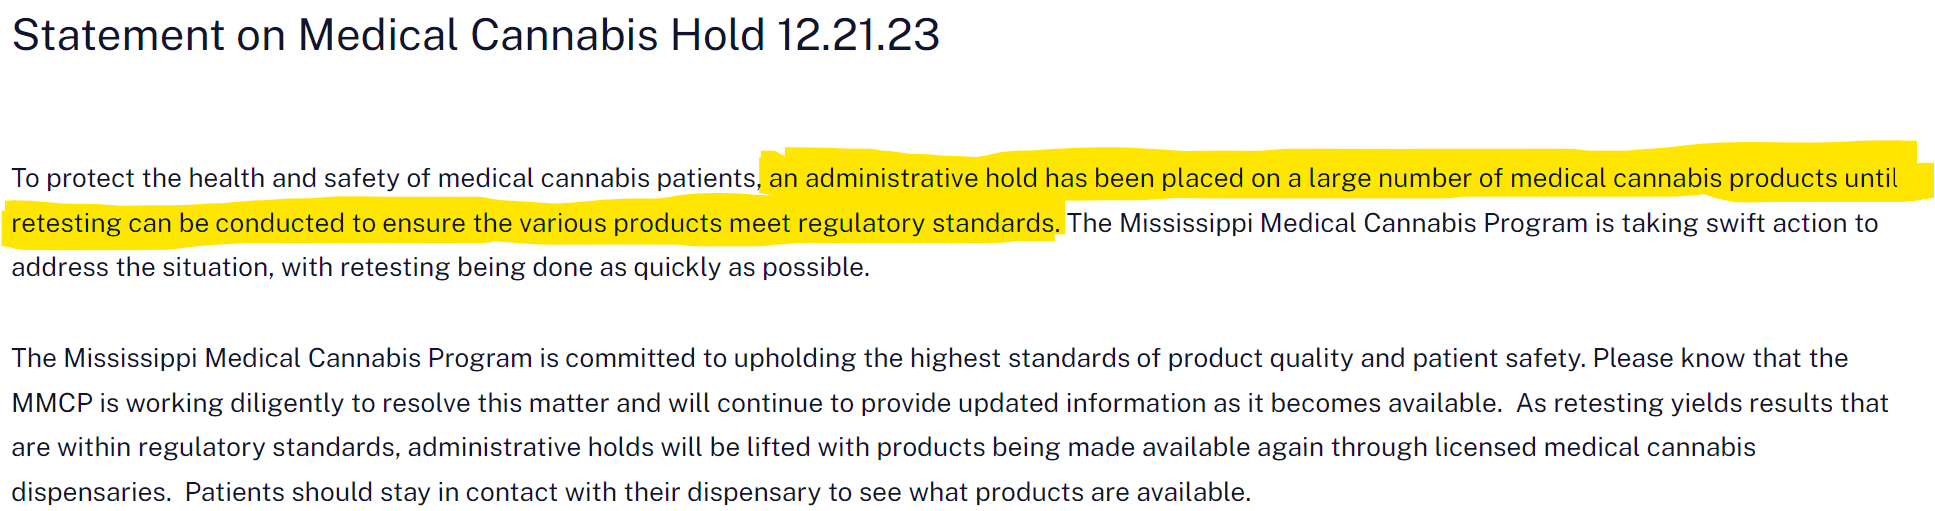
\includegraphics[width=1.1\textwidth]{images/ms-statement-1.png}
\end{center}
\vspace{4\baselineskip}
{\tiny Source: https://www.mmcp.ms.gov/?fbclid=IwAR1ncdtODhJquA5Z7l\_jiAP7kCJGu1\_T4YubosGM3dmAUM9msiw5oWaCf30}
\end{frame}

% Mississippi news bulletin
\begin{frame}{Mississippi News Bulletin Update  - 2023-12-21}
\begin{center}
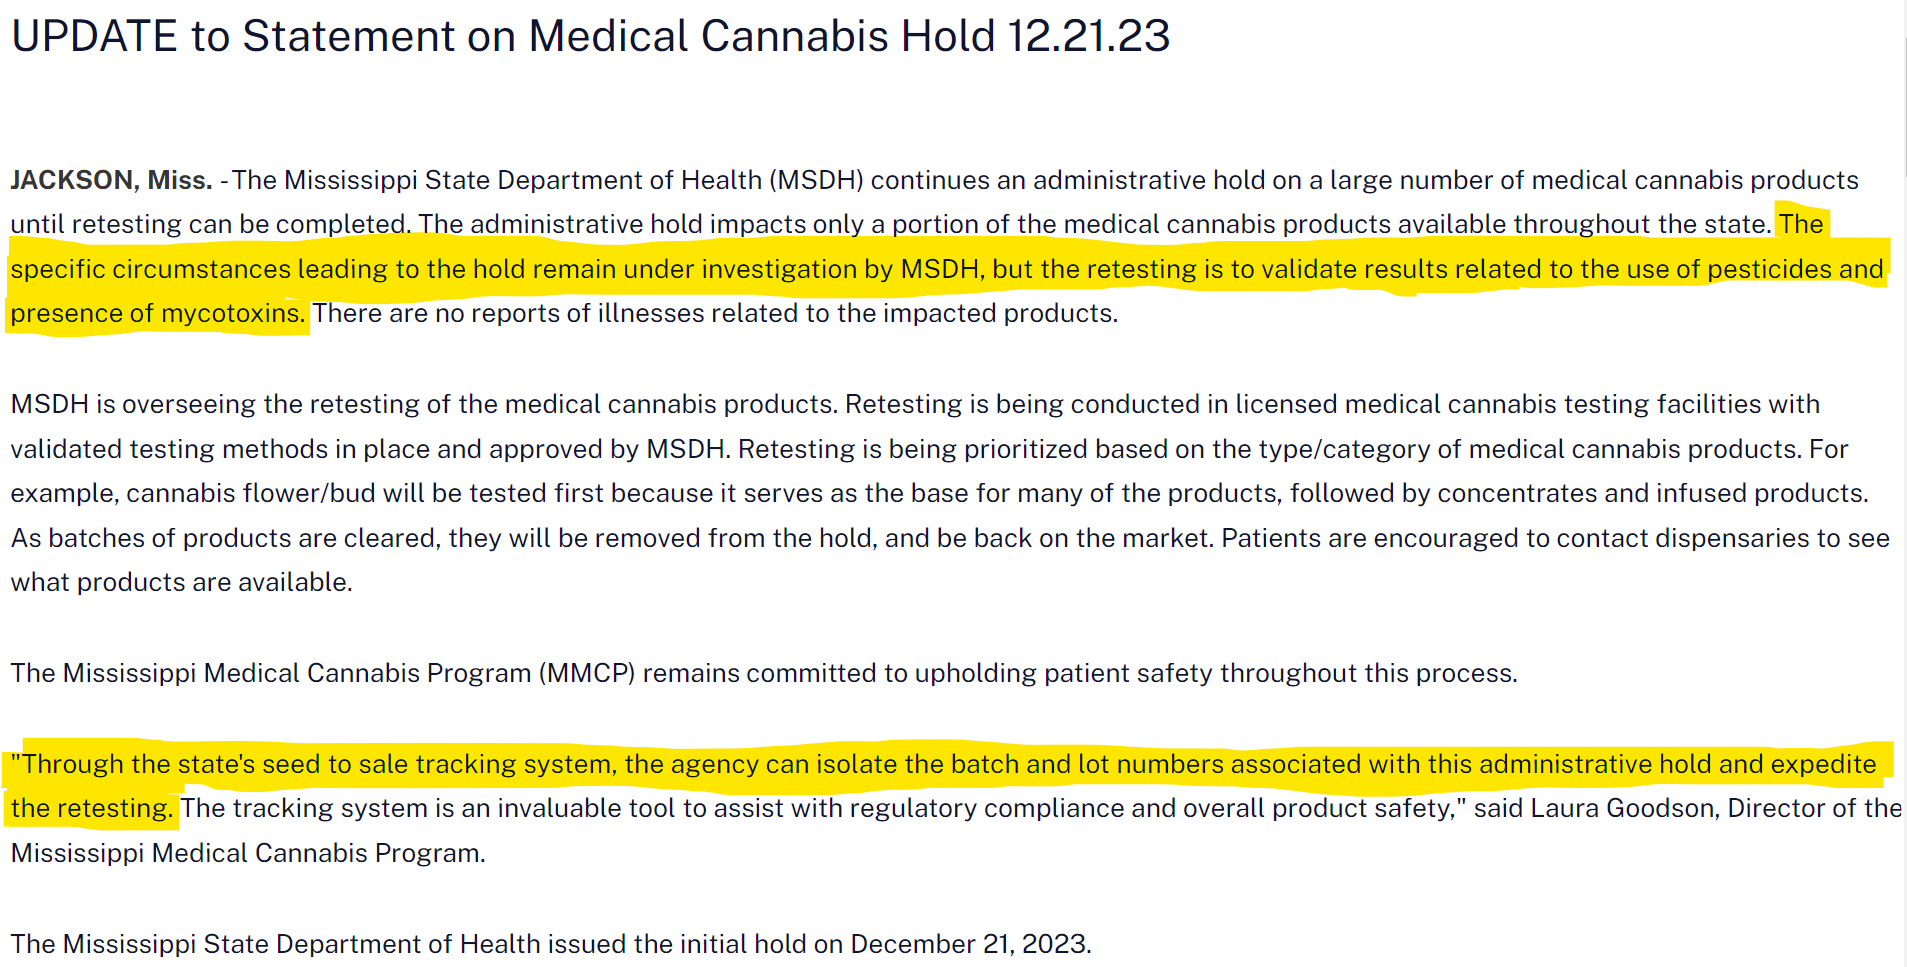
\includegraphics[width=1.1\textwidth]{images/ms-statement-2.png}
\end{center}
\vfill
{\tiny Source: https://www.mmcp.ms.gov/?fbclid=IwAR1ncdtODhJquA5Z7l\_jiAP7kCJGu1\_T4YubosGM3dmAUM9msiw5oWaCf30}
\end{frame}


% Marijuana moment article
\begin{frame}{Marijuana Moment Article - 2023-12-25}
\begin{center}
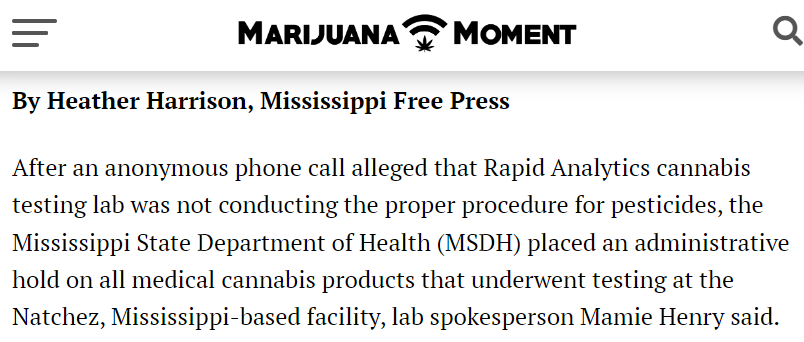
\includegraphics[width=1\textwidth]{images/mm-article-1.png}
\end{center}
\vfill
{\tiny Source: https://www.marijuanamoment.net/mississippi-regulators-place-hold-on-large-number-of-medical-marijuana-after-receiving-anonymous-call/}
\end{frame}


\begin{frame}
\begin{center}
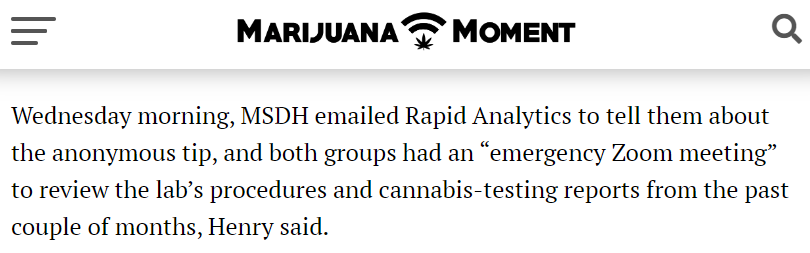
\includegraphics[width=1\textwidth]{images/mm-article-3.png}
\end{center}
\end{frame}

% Marijuana moment article
\begin{frame}
\begin{center}
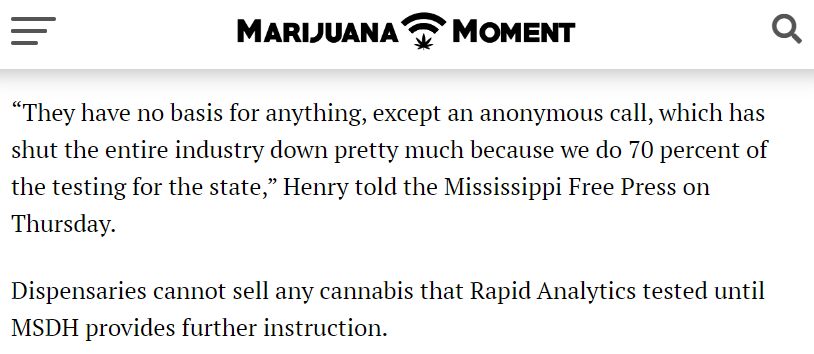
\includegraphics[width=1\textwidth]{images/mm-article-2.png}
%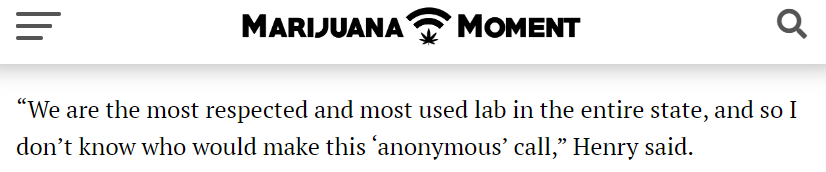
\includegraphics[width=1\textwidth]{images/mm-article-4.png}
\end{center}
\end{frame}

%\begin{frame}
%\begin{center}
%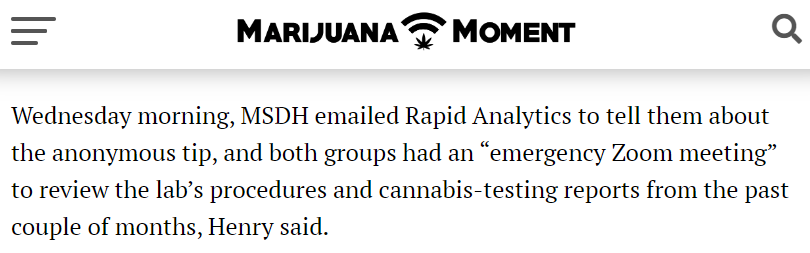
\includegraphics[width=1.1\textwidth]{images/mm-article-3.png}
%\end{center}
%\end{frame}


\begin{frame}
\begin{center}
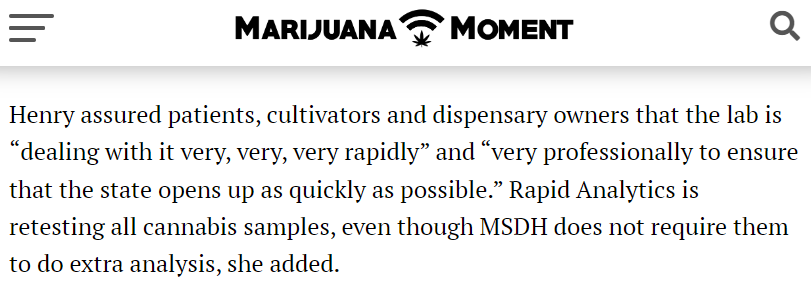
\includegraphics[width=1\textwidth]{images/mm-article-5.png}
\end{center}
\end{frame}

\begin{frame}
\begin{center}
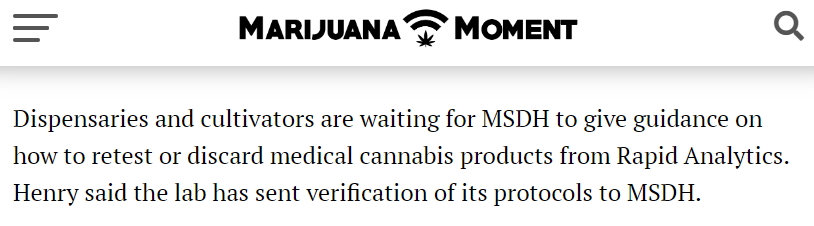
\includegraphics[width=1\textwidth]{images/mm-article-6.png}
\end{center}
\end{frame}


% Mississippi testing regulations
%\begin{frame}{Mississippi Pesticide Testing Regulations}
%\begin{center}
%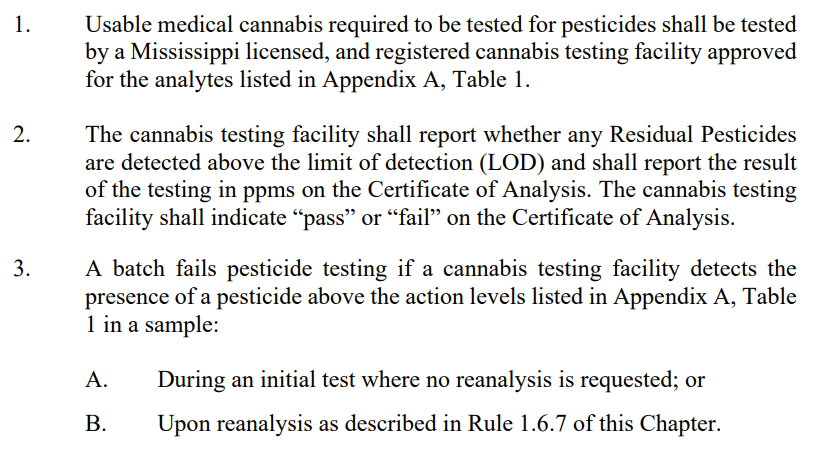
\includegraphics[width=\textwidth]{images/ms-pesticide-testing-rules.png}
%\end{center}
%{\tiny Data Source: https://www.mmcp.ms.gov/sites/default/files/Documents/Title15Part22Subpart1Testing.pdf}
%\end{frame}


% ms-pesticides-table-1
% ms-pesticides-table-2



%------------------------------------------%
% Data
%------------------------------------------%


\begin{frame}{Data}

\begin{itemize}


\item Population of Mississippi: 2,938,928 (2022)

\vspace*{\baselineskip}

\item Population of Connecticut: 3,617,176 (2022)

\end{itemize}

\vfill

{\tiny Data Source: https://www.census.gov/quickfacts/CT}


\end{frame}


%------------------------------------------%
% Mississippi Market Analysis
%------------------------------------------%

% Introduce MS data.


% Retailers per capita in MS map.
\begin{frame}{Dispensaries per 100,000 people by county in Mississippi}

\begin{center}
\includegraphics[width=0.4\textwidth]{images/ms-retailers-per-capita-map-2023-12-28.pdf}
\end{center}

\end{frame}


% Retailers per capita in MS bar chart.
\begin{frame}

\begin{center}
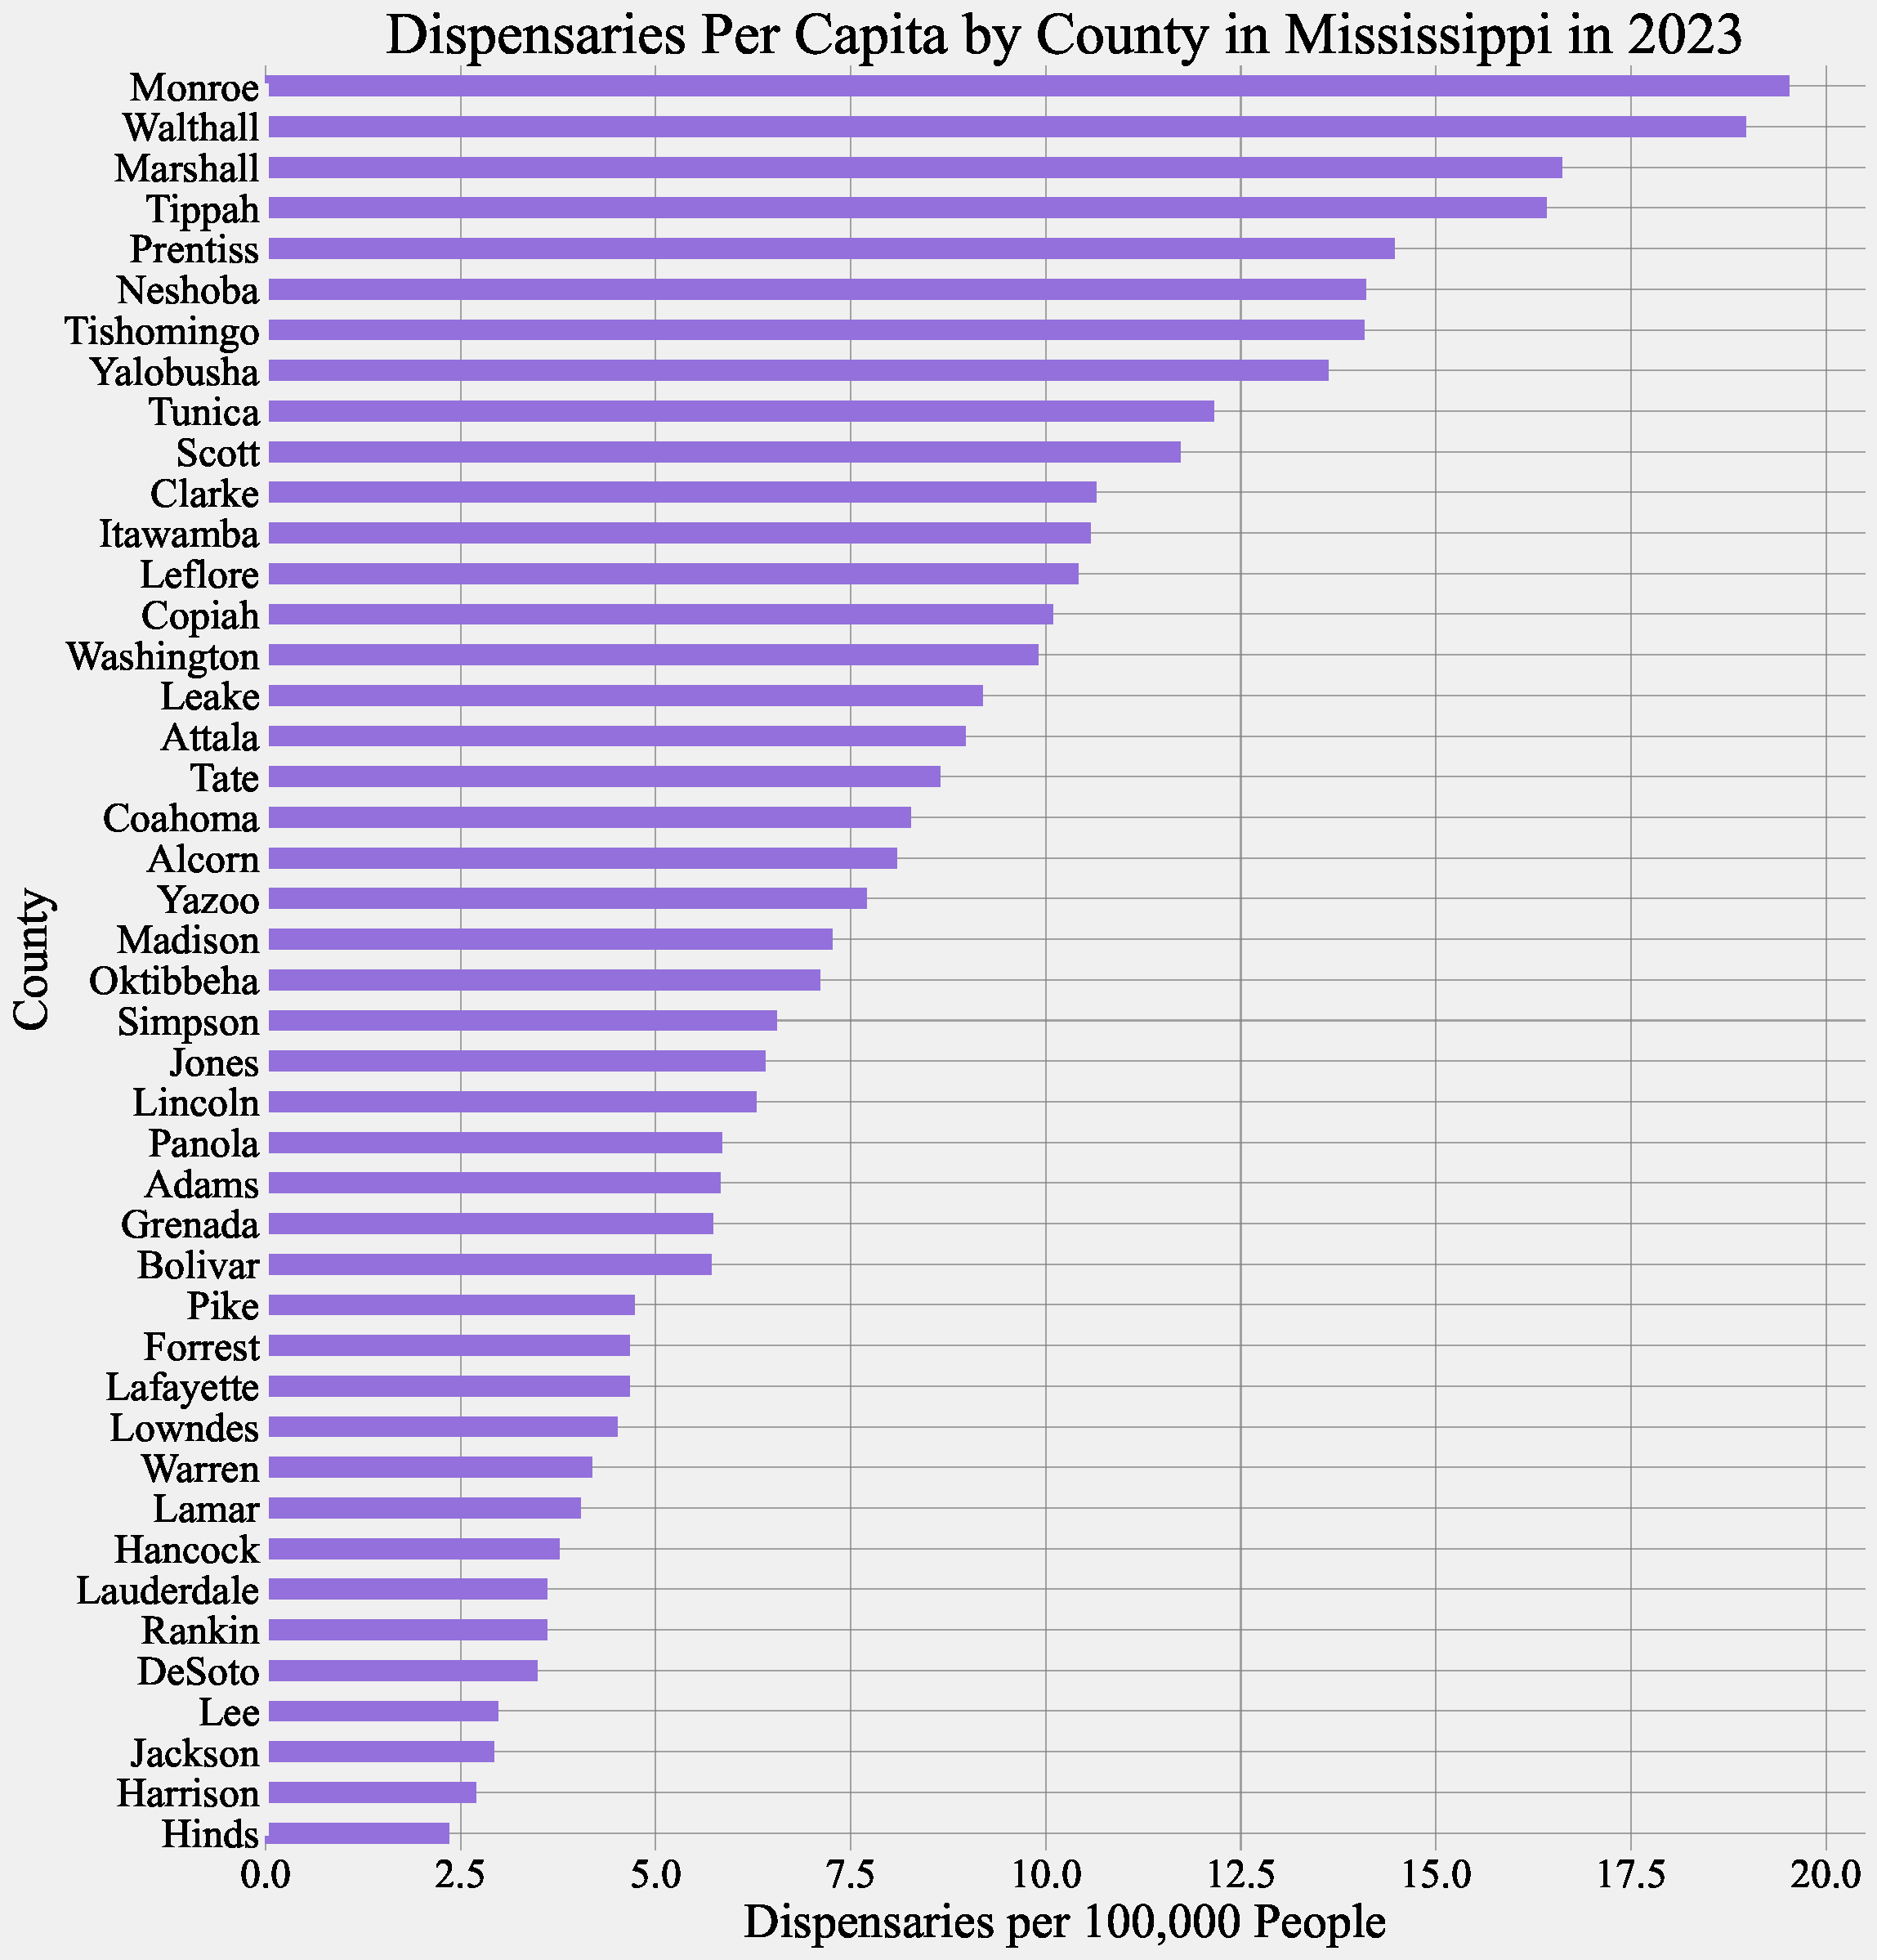
\includegraphics[width=0.75\textwidth]{images/ms-retailers-per-capita-2023-12-28.pdf}
\end{center}

\end{frame}



%------------------------------------------%
% Connecticut news articles
%------------------------------------------%

\begin{frame}
\begin{center}
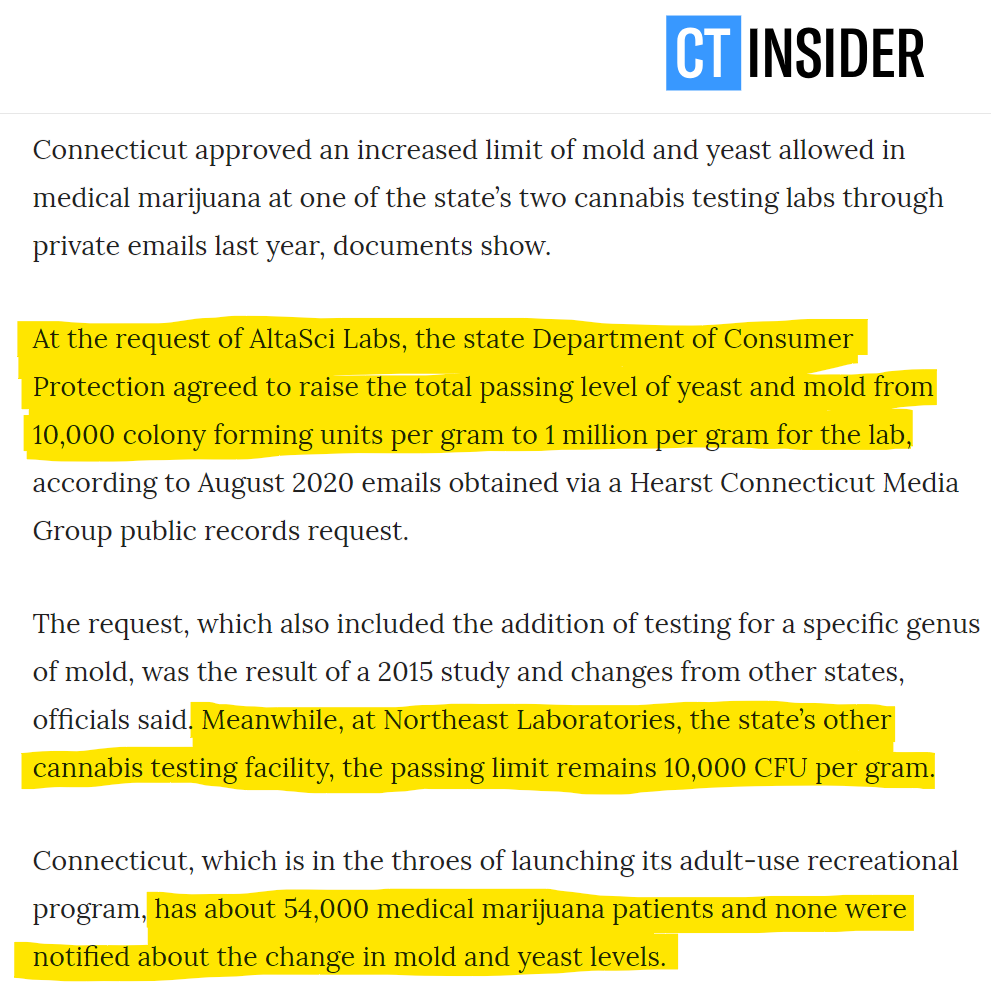
\includegraphics[width=0.75\textwidth]{images/ct-article-3.png}
\end{center}
{\tiny Source: https://www.ctinsider.com/news/article/Connecticut-raises-mold-levels-for-medical-16678474.php }
\end{frame}

\begin{frame}
\begin{center}
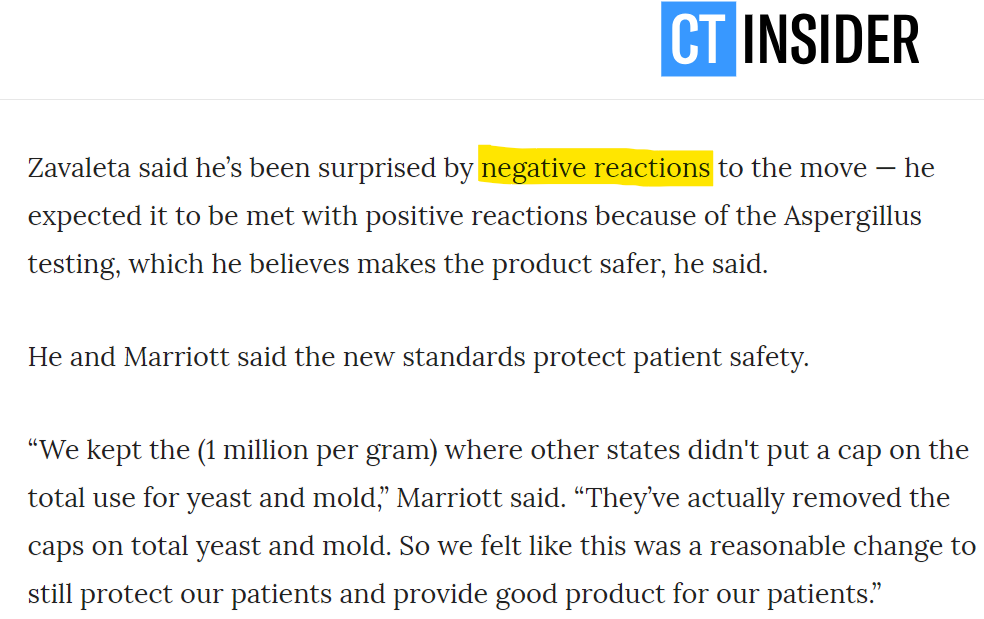
\includegraphics[width=1\textwidth]{images/ct-article-1.png}
\end{center}
\end{frame}

\begin{frame}
\begin{center}
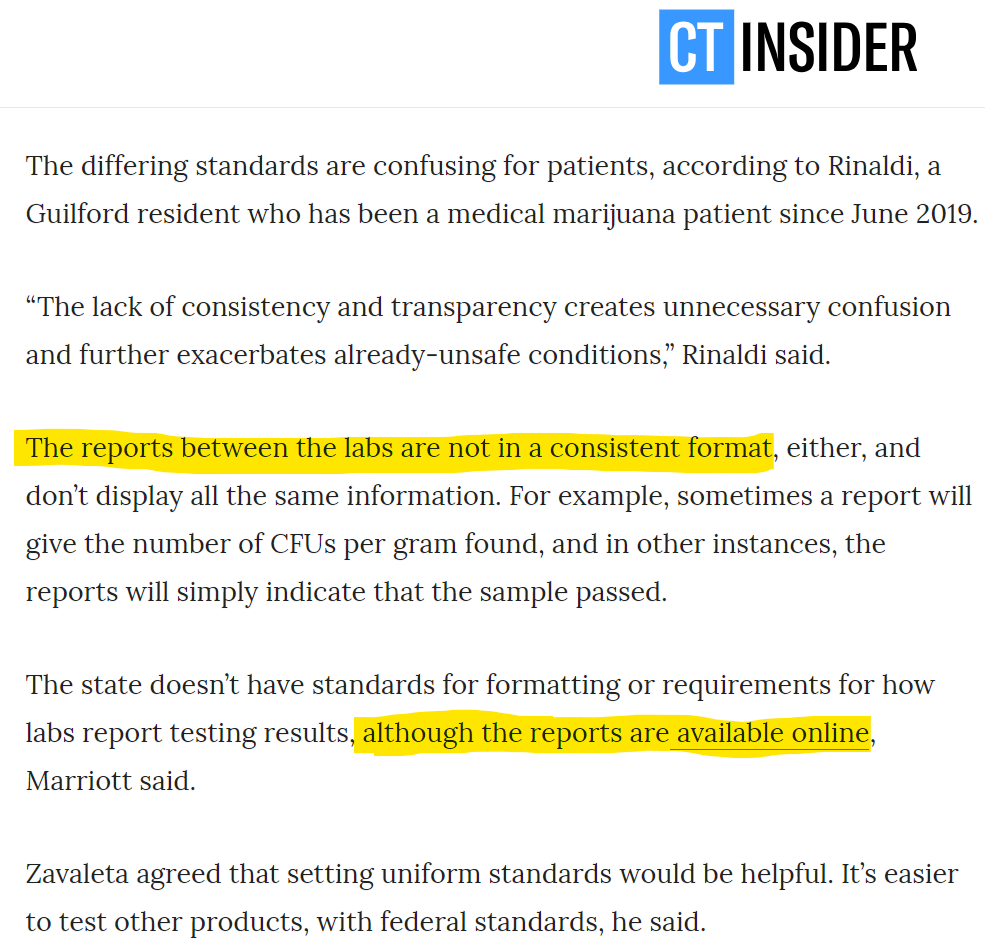
\includegraphics[width=0.8\textwidth]{images/ct-article-2.png}
\end{center}
\end{frame}


%------------------------------------------%
% Connecticut Market Analysis
%------------------------------------------%

% Introduce Connecticut data.


% Lab tests in CT.
\begin{frame}
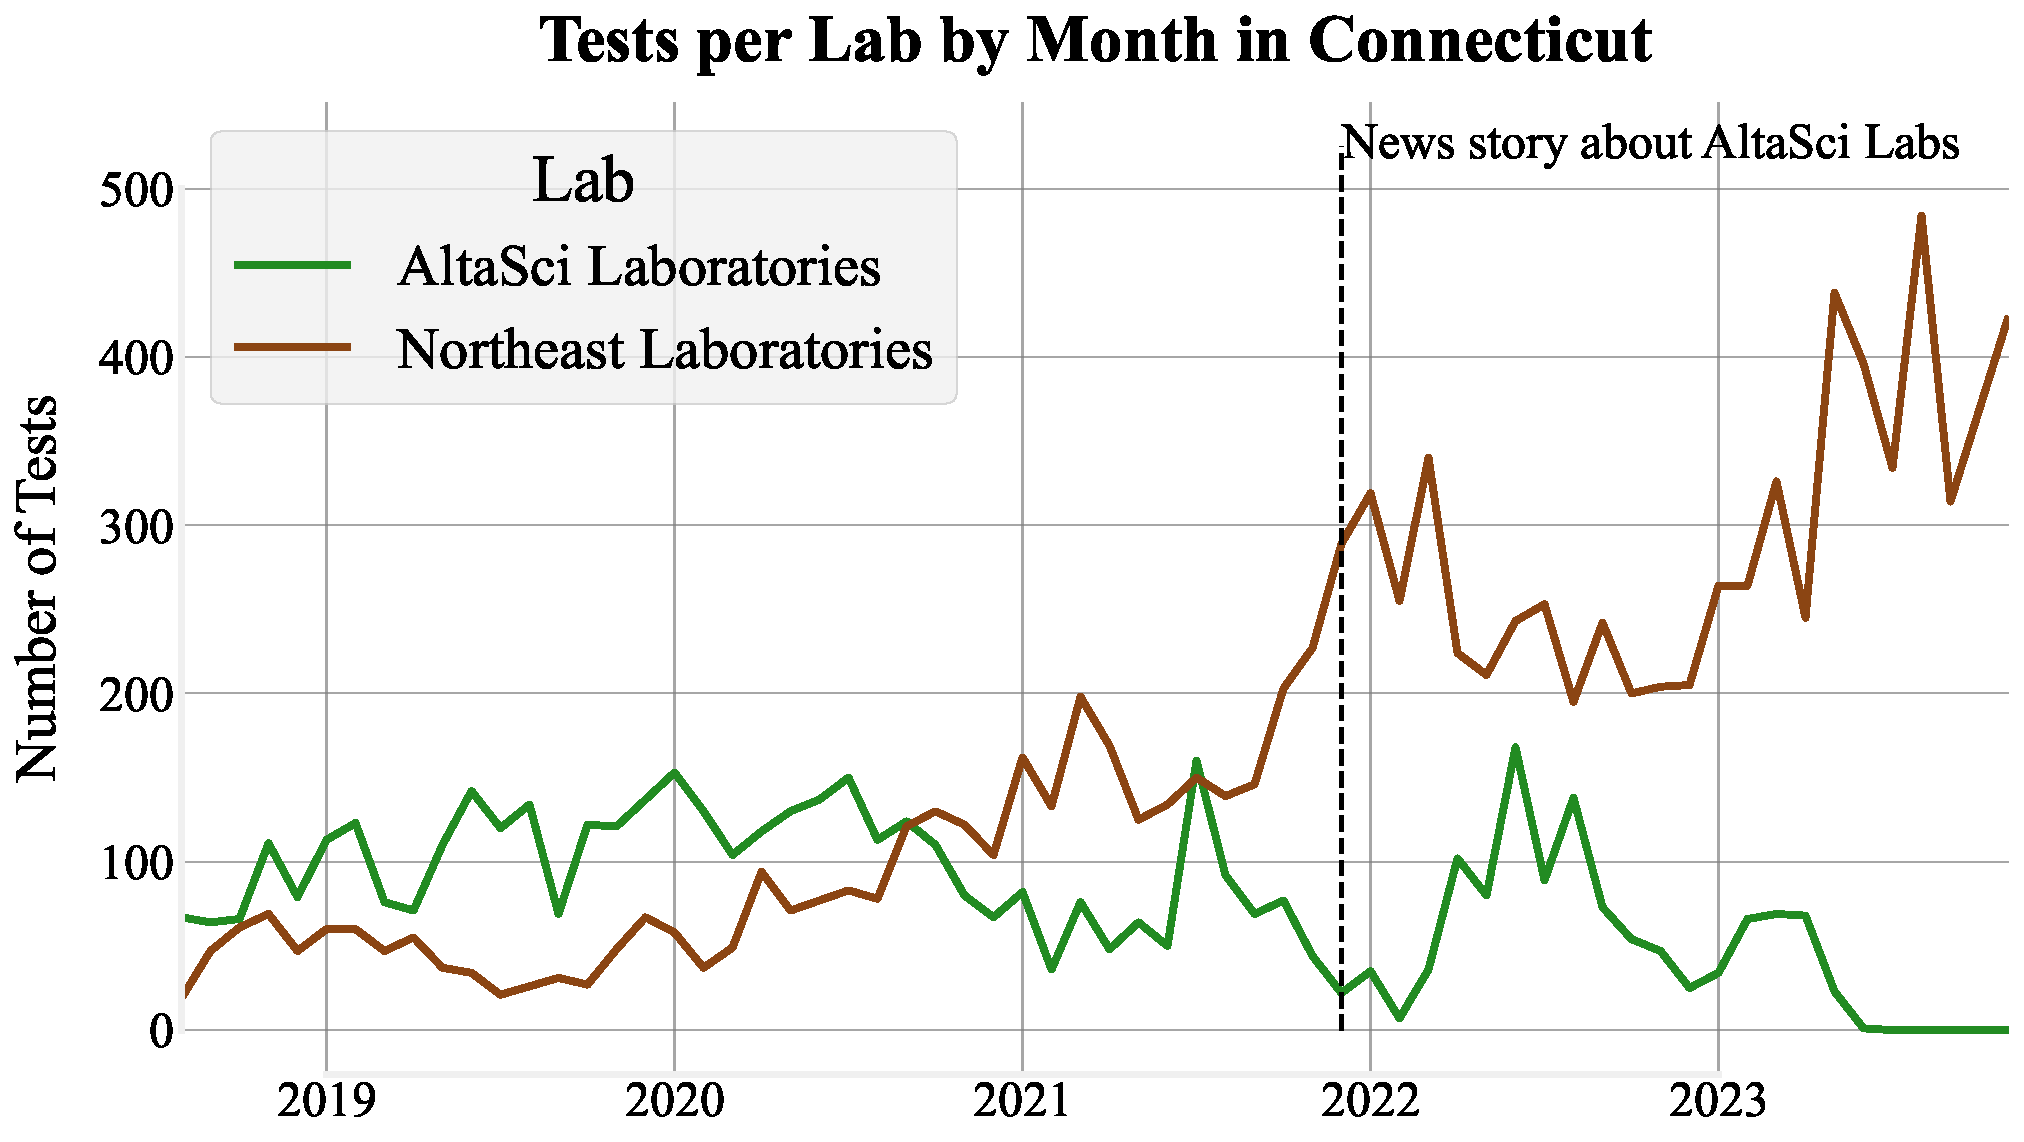
\includegraphics[width=\textwidth]{images/ct-tests-per-lab-per-month.pdf}
\end{frame}


% Lab market share in CT.
\begin{frame}
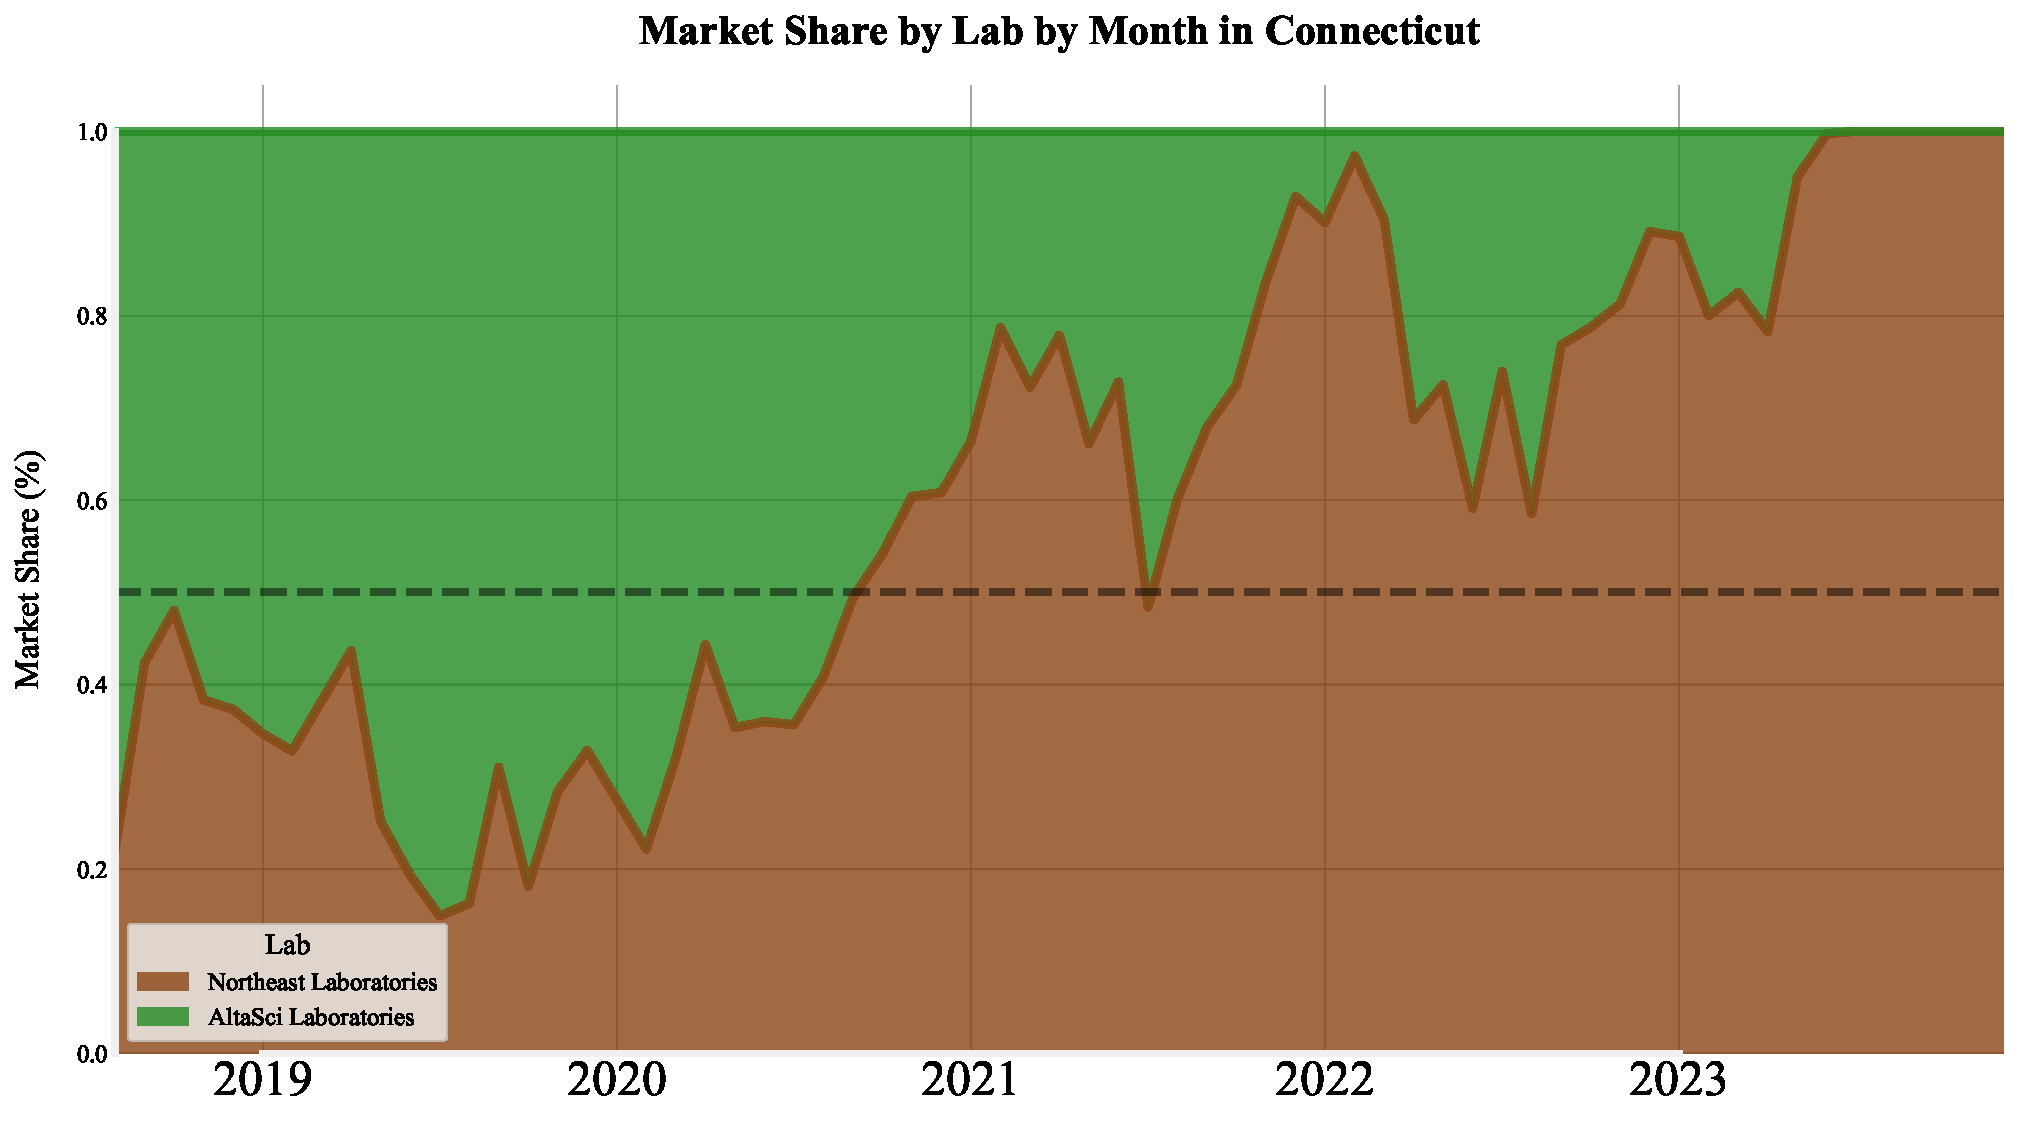
\includegraphics[width=\textwidth]{images/ct-market-share-per-lab-per-month.pdf}

\end{frame}


%------------------------------------------%
% Lab Analysis
%------------------------------------------%


% Turnaround time by lab.


% Analysis of reviewers.




%------------------------------------------%
% Takeaway
%------------------------------------------%
\section{Takeaway}
\begin{frame}{}

\begin{center}
\begin{minipage}{3.85in}

% Thank you.

\includegraphics[width=.25in]{images/prayer.png} {\Large \textbf{Thank you for coming.}}\\

% Re-cap the lesson of the week.
\begin{center}
\begin{minipage}{.9\linewidth}
\begin{Block}{Lessons of the Day}

\vspace{\baselineskip}

\begin{itemize}

\item What happens early happens often.

\vspace{\baselineskip}

\end{itemize}

\end{Block}
\end{minipage}
\end{center}

\vfill

\end{minipage}
\end{center}

\end{frame}


%------------------------------------------%
% End
%------------------------------------------%
\end{document}
